\documentclass[11pt]{article}

\newcommand{\titrechapitre}{Vecteurs -- Exercices}
\newcommand{\titreclasse}{Lycée Jean-Baptiste \textsc{Corot}}
\newcommand{\pagination}{\thepage/\pageref{LastPage}}
\newcommand{\topbotmargins}{1.5cm}
\newcommand{\spacebelowexo}{1mm}

%%%%%%%%%%%%%%%%%%%%%%%%%%%%%%%%%%%%%%%%%%%%%%%%%%%%%%%%%%%%%%%%%%%%%%%%%%%%%%%%
%
% PACKAGES
% ========
%
%%%%%%%%%%%%%%%%%%%%%%%%%%%%%%%%%%%%%%%%%%%%%%%%%%%%%%%%%%%%%%%%%%%%%%%%%%%%%%%%

\usepackage[english, french]{babel}
\usepackage[utf8]{inputenc}
\usepackage[T1]{fontenc}
\usepackage{graphicx}
\usepackage{amsmath,amssymb,amsthm,amsopn}
\usepackage{hyperref}

% Pour avoir l'écriture \mathscr (math script)
% ============================================

\usepackage{mathrsfs}

% Deal with coma as a decimal separator
% =====================================

\usepackage{icomma}

% Package Geometry
% ================

\usepackage[a4paper, lmargin=2cm, rmargin=2cm, top=\topbotmargins, bottom=\topbotmargins]{geometry}

% Package multicol
% ================

\usepackage{multicol}

% Redefine abstract
% =================

% Note
% ====
%
% Le reste a été commenté pour ne pas charger trop de choses au démarrage. On
% verra si on en a besoin plus tard.
%
% --------
%
%\usepackage{mathrsfs}
%\usepackage{multirow}
%\usepackage{bm}
%\hypersetup{
%    colorlinks=true,
%    linkcolor=blue,
%    citecolor=red,
%}
%\usepackage{diagbox}
%
%\usepackage{algorithm}
%\usepackage{algpseudocode}
%
%\renewcommand{\algorithmicrequire}{\textbf{Input:}}
%\renewcommand{\algorithmicensure}{\textbf{Output:}}


%%%%%%%%%%%%%%%%%%%%%%%%%%%%%%%%%%%%%%%%%%%%%%%%%%%%%%%%%%%%%%%%%%%%%%%%%%%%%%%%
%
% TIKZ
% ====
%
%%%%%%%%%%%%%%%%%%%%%%%%%%%%%%%%%%%%%%%%%%%%%%%%%%%%%%%%%%%%%%%%%%%%%%%%%%%%%%%%

\usepackage{tikz}
\usetikzlibrary{arrows}

\usepackage{tkz-tab} % Variation tables

\usepackage{pgfplots}
%\usepackage{pgf-pie} % Pie charts

\pgfplotsset{
%\newcommand{\settingsgraph}{
x=.5cm,y=.5cm,
xticklabel style = {font=\scriptsize, yshift=.1cm},
yticklabel style = {font=\scriptsize, xshift=.1cm},
axis lines=middle,
ymajorgrids=true,
xmajorgrids=true,
major grid style = {color=white!80!blue},
xmin=-5.5,
xmax=5.5,
ymin=-5.5,
ymax=5.5,
xtick={-5.0,-4.0,...,5.0},
ytick={-5.0,-4.0,...,5.0},
}

% Tikz style

\tikzset{round/.style={circle, draw=black, very thick, scale = 0.7}}
\tikzset{arrow/.style={->, >=latex}}
\tikzset{dashed-arrow/.style={->, >=latex, dashed}}

\newcommand{\point}[3]{\draw[very thick, #3] (#1-.1, #2)--(#1+.1, #2)
(#1, #2-.1)--(#1, #2+.1)}

%%%%%%%%%%%%%%%%%%%%%%%%%%%%%%%%%%%%%%%%%%%%%%%%%%%%%%%%%%%%%%%%%%%%%%%%%%%%%%%%
%
% FANCY HEADER
% ============
%
%%%%%%%%%%%%%%%%%%%%%%%%%%%%%%%%%%%%%%%%%%%%%%%%%%%%%%%%%%%%%%%%%%%%%%%%%%%%%%%%


\usepackage{fancyhdr}
\usepackage{lastpage}

\pagestyle{fancy}
\newcommand{\changefont}{\fontsize{9}{9}\selectfont}
\renewcommand{\headrulewidth}{0mm}
\renewcommand{\footrulewidth}{0mm}

\fancyhead[C]{}
\fancyhead[L]{\titreclasse}
\fancyhead[R]{\titrechapitre}
\fancyfoot[C]{}
\fancyfoot[L]{}
\fancyfoot[R]{\pagination}
\addtolength{\skip\footins}{20pt} % distance between text and footnotes

%%%%%%%%%%%%%%%%%%%%%%%%%%%%%%%%%%%%%%%%%%%%%%%%%%%%%%%%%%%%%%%%%%%%%%%%%%%%%%%%
%
% THEOREM STYLE
% =============
%
%%%%%%%%%%%%%%%%%%%%%%%%%%%%%%%%%%%%%%%%%%%%%%%%%%%%%%%%%%%%%%%%%%%%%%%%%%%%%%%%

\usepackage[tikz]{bclogo}
\usepackage{mdframed}

\usepackage{tcolorbox}
\tcbuselibrary{listings, breakable, theorems, skins}

%\newtheoremstyle{break}%
%{}{}%
%{\itshape}{}%
%{\bfseries}{}%  % Note that final punctuation is omitted.
%{\newline}{}

\newtheoremstyle{scbf}%
{}{}%
{}{}%
%{\scshape}{}%  % Note that final punctuation is omitted.
{\bfseries\scshape}{}%  % Note that final punctuation is omitted.
{\newline}{}

%\theoremstyle{break}
%\theoremstyle{plain}
%\newtheorem{thm}{Theorem}[section]
%\newtheorem{lm}[thm]{Lemma}
%\newtheorem{prop}[thm]{Proposition}
%\newtheorem{cor}[thm]{Corollary}

%\theoremstyle{scbf}
%\newtheorem{exo}{$\star$ Exercice}

%\theoremstyle{definition}
%\newtheorem{defi}[thm]{Definition}
%\newtheorem{ex}[thm]{Example}

%\theoremstyle{remark}
%\newtheorem{rem}[thm]{Remark}

% Defining the Remark environment
% ===============================

\newenvironment{rmq}
  {
    \begin{bclogo}[logo=\bcinfo, noborder=true]{Remarque}
  }
  {
    \end{bclogo}
  }

% Defining the exercise environment
% =================================

\newcounter{exos}
\setcounter{exos}{1}

\newenvironment{exo}
  {
    \begin{bclogo}[logo=\bccrayon, noborder=true]{Exercice \theexos}
  }
  {
    \end{bclogo}
    \addtocounter{exos}{1}
  }


% Redefining the proof environment from amsthm
% ============================================

\tcolorboxenvironment{proof}{
  blanker, breakable, before skip=10pt,after skip=10pt,
  borderline west={1mm}{0pt}{red},
  left=5mm,
}

% Defining the definition environment
% ===================================

\colorlet{coldef}{black!50!green}

\newcounter{defis}
\setcounter{defis}{1}

\newenvironment{defi}[1]
  {
    \begin{defihid}{{#1}}{\thedefis}
  }
  {
    \end{defihid}
    \addtocounter{defis}{1}
  }

\newtcolorbox{defihid}[2]{%
  empty,title={ {\bfseries Définition {#2}} ({#1})},attach boxed title to top left,
boxed title style={empty,size=minimal,toprule=2pt,top=4pt,
overlay={\draw[coldef,line width=2pt]
([yshift=-1pt]frame.north west)--([yshift=-1pt]frame.north east);}},
coltitle=coldef,
before=\par\medskip\noindent,parbox=false,boxsep=0pt,left=0pt,right=3mm,top=4pt,
breakable,pad at break*=0mm,vfill before first,
overlay unbroken={\draw[coldef,line width=1pt]
([yshift=-1pt]title.north east)--([xshift=-0.5pt,yshift=-1pt]title.north-|frame.east)
--([xshift=-0.5pt]frame.south east)--(frame.south west); },
overlay first={\draw[coldef,line width=1pt]
([yshift=-1pt]title.north east)--([xshift=-0.5pt,yshift=-1pt]title.north-|frame.east)
--([xshift=-0.5pt]frame.south east); },
overlay middle={\draw[coldef,line width=1pt] ([xshift=-0.5pt]frame.north east)
--([xshift=-0.5pt]frame.south east); },
overlay last={\draw[coldef,line width=1pt] ([xshift=-0.5pt]frame.north east)
--([xshift=-0.5pt]frame.south east)--(frame.south west);},%
}

\newenvironment{notation}
  {
    \begin{notationhid}{\thedefis}
  }
  {
    \end{notationhid}
    \addtocounter{defis}{1}
  }

\newtcolorbox{notationhid}[1]{%
  empty,title={Notation {#1}},attach boxed title to top left,
boxed title style={empty,size=minimal,toprule=2pt,top=4pt,
overlay={\draw[coldef,line width=2pt]
([yshift=-1pt]frame.north west)--([yshift=-1pt]frame.north east);}},
coltitle=coldef,fonttitle=\bfseries,
before=\par\medskip\noindent,parbox=false,boxsep=0pt,left=0pt,right=3mm,top=4pt,
breakable,pad at break*=0mm,vfill before first,
overlay unbroken={\draw[coldef,line width=1pt]
([yshift=-1pt]title.north east)--([xshift=-0.5pt,yshift=-1pt]title.north-|frame.east)
--([xshift=-0.5pt]frame.south east)--(frame.south west); },
overlay first={\draw[coldef,line width=1pt]
([yshift=-1pt]title.north east)--([xshift=-0.5pt,yshift=-1pt]title.north-|frame.east)
--([xshift=-0.5pt]frame.south east); },
overlay middle={\draw[coldef,line width=1pt] ([xshift=-0.5pt]frame.north east)
--([xshift=-0.5pt]frame.south east); },
overlay last={\draw[coldef,line width=1pt] ([xshift=-0.5pt]frame.north east)
--([xshift=-0.5pt]frame.south east)--(frame.south west);},%
}


% Defining the proposition, theorem, etc. environment
% ===================================================

\colorlet{colprop}{red!75!black}

\newcounter{props}
\setcounter{props}{1}

\newenvironment{prop}
  {
    \begin{prophid}{\theprops}
  }
  {
    \end{prophid}
    \refstepcounter{props}
  }

\newtcolorbox{prophid}[1]{%
empty,title={Propriété {#1}},attach boxed title to top left,
boxed title style={empty,size=minimal,toprule=2pt,top=4pt,
overlay={\draw[colprop,line width=2pt]
([yshift=-1pt]frame.north west)--([yshift=-1pt]frame.north east);}},
coltitle=colprop,fonttitle=\bfseries,
before=\par\medskip\noindent,parbox=false,boxsep=0pt,left=0pt,right=3mm,top=4pt,
breakable,pad at break*=0mm,vfill before first,
overlay unbroken={\draw[colprop,line width=1pt]
([yshift=-1pt]title.north east)--([xshift=-0.5pt,yshift=-1pt]title.north-|frame.east)
--([xshift=-0.5pt]frame.south east)--(frame.south west); },
overlay first={\draw[colprop,line width=1pt]
([yshift=-1pt]title.north east)--([xshift=-0.5pt,yshift=-1pt]title.north-|frame.east)
--([xshift=-0.5pt]frame.south east); },
overlay middle={\draw[colprop,line width=1pt] ([xshift=-0.5pt]frame.north east)
--([xshift=-0.5pt]frame.south east); },
overlay last={\draw[colprop,line width=1pt] ([xshift=-0.5pt]frame.north east)
--([xshift=-0.5pt]frame.south east)--(frame.south west);},%
}

\newenvironment{propadm}
  {
    \begin{propadmhid}{\theprops}
  }
  {
    \end{propadmhid}
    \refstepcounter{props}
  }

  \newtcolorbox{propadmhid}[1]{%
    empty,title={{\bfseries Propriété {#1}} (admise)},attach boxed title to top left,
boxed title style={empty,size=minimal,toprule=2pt,top=4pt,
overlay={\draw[colprop,line width=2pt]
([yshift=-1pt]frame.north west)--([yshift=-1pt]frame.north east);}},
coltitle=colprop,%fonttitle=\bfseries,
before=\par\medskip\noindent,parbox=false,boxsep=0pt,left=0pt,right=3mm,top=4pt,
breakable,pad at break*=0mm,vfill before first,
overlay unbroken={\draw[colprop,line width=1pt]
([yshift=-1pt]title.north east)--([xshift=-0.5pt,yshift=-1pt]title.north-|frame.east)
--([xshift=-0.5pt]frame.south east)--(frame.south west); },
overlay first={\draw[colprop,line width=1pt]
([yshift=-1pt]title.north east)--([xshift=-0.5pt,yshift=-1pt]title.north-|frame.east)
--([xshift=-0.5pt]frame.south east); },
overlay middle={\draw[colprop,line width=1pt] ([xshift=-0.5pt]frame.north east)
--([xshift=-0.5pt]frame.south east); },
overlay last={\draw[colprop,line width=1pt] ([xshift=-0.5pt]frame.north east)
--([xshift=-0.5pt]frame.south east)--(frame.south west);},%
}

\newenvironment{propnom}[1]
  {
    \begin{propnomhid}{#1}{\theprops}
  }
  {
    \end{propnomhid}
    \refstepcounter{props}
  }

\newtcolorbox{propnomhid}[2]{%
empty,title={{\bfseries Propriété {#2}} ({#1})},attach boxed title to top left,
boxed title style={empty,size=minimal,toprule=2pt,top=4pt,
overlay={\draw[colprop,line width=2pt]
([yshift=-1pt]frame.north west)--([yshift=-1pt]frame.north east);}},
coltitle=colprop,
before=\par\medskip\noindent,parbox=false,boxsep=0pt,left=0pt,right=3mm,top=4pt,
breakable,pad at break*=0mm,vfill before first,
overlay unbroken={\draw[colprop,line width=1pt]
([yshift=-1pt]title.north east)--([xshift=-0.5pt,yshift=-1pt]title.north-|frame.east)
--([xshift=-0.5pt]frame.south east)--(frame.south west); },
overlay first={\draw[colprop,line width=1pt]
([yshift=-1pt]title.north east)--([xshift=-0.5pt,yshift=-1pt]title.north-|frame.east)
--([xshift=-0.5pt]frame.south east); },
overlay middle={\draw[colprop,line width=1pt] ([xshift=-0.5pt]frame.north east)
--([xshift=-0.5pt]frame.south east); },
overlay last={\draw[colprop,line width=1pt] ([xshift=-0.5pt]frame.north east)
--([xshift=-0.5pt]frame.south east)--(frame.south west);},%
}




\newenvironment{thm}
  {
    \begin{thmhid}{\theprops}
  }
  {
    \end{thmhid}
    \refstepcounter{props}
  }

\newtcolorbox{thmhid}[1]{%
empty,title={Théorème {#1}},attach boxed title to top left,
boxed title style={empty,size=minimal,toprule=2pt,top=4pt,
overlay={\draw[colprop,line width=2pt]
([yshift=-1pt]frame.north west)--([yshift=-1pt]frame.north east);}},
coltitle=colprop,fonttitle=\bfseries,
before=\par\medskip\noindent,parbox=false,boxsep=0pt,left=0pt,right=3mm,top=4pt,
breakable,pad at break*=0mm,vfill before first,
overlay unbroken={\draw[colprop,line width=1pt]
([yshift=-1pt]title.north east)--([xshift=-0.5pt,yshift=-1pt]title.north-|frame.east)
--([xshift=-0.5pt]frame.south east)--(frame.south west); },
overlay first={\draw[colprop,line width=1pt]
([yshift=-1pt]title.north east)--([xshift=-0.5pt,yshift=-1pt]title.north-|frame.east)
--([xshift=-0.5pt]frame.south east); },
overlay middle={\draw[colprop,line width=1pt] ([xshift=-0.5pt]frame.north east)
--([xshift=-0.5pt]frame.south east); },
overlay last={\draw[colprop,line width=1pt] ([xshift=-0.5pt]frame.north east)
--([xshift=-0.5pt]frame.south east)--(frame.south west);},%
}

\newenvironment{thmadm}
  {
    \begin{thmadmhid}{\theprops}
  }
  {
    \end{thmadmhid}
    \refstepcounter{props}
  }

  \newtcolorbox{thmadmhid}[1]{%
    empty,title={{\bfseries Théorème {#1}} (admis)},attach boxed title to top left,
boxed title style={empty,size=minimal,toprule=2pt,top=4pt,
overlay={\draw[colprop,line width=2pt]
([yshift=-1pt]frame.north west)--([yshift=-1pt]frame.north east);}},
coltitle=colprop,%fonttitle=\bfseries,
before=\par\medskip\noindent,parbox=false,boxsep=0pt,left=0pt,right=3mm,top=4pt,
breakable,pad at break*=0mm,vfill before first,
overlay unbroken={\draw[colprop,line width=1pt]
([yshift=-1pt]title.north east)--([xshift=-0.5pt,yshift=-1pt]title.north-|frame.east)
--([xshift=-0.5pt]frame.south east)--(frame.south west); },
overlay first={\draw[colprop,line width=1pt]
([yshift=-1pt]title.north east)--([xshift=-0.5pt,yshift=-1pt]title.north-|frame.east)
--([xshift=-0.5pt]frame.south east); },
overlay middle={\draw[colprop,line width=1pt] ([xshift=-0.5pt]frame.north east)
--([xshift=-0.5pt]frame.south east); },
overlay last={\draw[colprop,line width=1pt] ([xshift=-0.5pt]frame.north east)
--([xshift=-0.5pt]frame.south east)--(frame.south west);},%
}

\newenvironment{thmnom}[1]
  {
    \begin{thmnomhid}{#1}{\theprops}
  }
  {
    \end{thmnomhid}
    \refstepcounter{props}
  }

\newtcolorbox{thmnomhid}[2]{%
empty,title={{\bfseries Théorème {#2}} ({#1})},attach boxed title to top left,
boxed title style={empty,size=minimal,toprule=2pt,top=4pt,
overlay={\draw[colprop,line width=2pt]
([yshift=-1pt]frame.north west)--([yshift=-1pt]frame.north east);}},
coltitle=colprop,
before=\par\medskip\noindent,parbox=false,boxsep=0pt,left=0pt,right=3mm,top=4pt,
breakable,pad at break*=0mm,vfill before first,
overlay unbroken={\draw[colprop,line width=1pt]
([yshift=-1pt]title.north east)--([xshift=-0.5pt,yshift=-1pt]title.north-|frame.east)
--([xshift=-0.5pt]frame.south east)--(frame.south west); },
overlay first={\draw[colprop,line width=1pt]
([yshift=-1pt]title.north east)--([xshift=-0.5pt,yshift=-1pt]title.north-|frame.east)
--([xshift=-0.5pt]frame.south east); },
overlay middle={\draw[colprop,line width=1pt] ([xshift=-0.5pt]frame.north east)
--([xshift=-0.5pt]frame.south east); },
overlay last={\draw[colprop,line width=1pt] ([xshift=-0.5pt]frame.north east)
--([xshift=-0.5pt]frame.south east)--(frame.south west);},%
}

\newenvironment{coro}
  {
    \begin{corohid}{\theprops}
  }
  {
    \end{corohid}
    \refstepcounter{props}
  }

  \newtcolorbox{corohid}[1]{%
  empty,title={Corollaire {#1}},attach boxed title to top left,
boxed title style={empty,size=minimal,toprule=2pt,top=4pt,
overlay={\draw[colprop,line width=2pt]
([yshift=-1pt]frame.north west)--([yshift=-1pt]frame.north east);}},
coltitle=colprop,fonttitle=\bfseries,
before=\par\medskip\noindent,parbox=false,boxsep=0pt,left=0pt,right=3mm,top=4pt,
breakable,pad at break*=0mm,vfill before first,
overlay unbroken={\draw[colprop,line width=1pt]
([yshift=-1pt]title.north east)--([xshift=-0.5pt,yshift=-1pt]title.north-|frame.east)
--([xshift=-0.5pt]frame.south east)--(frame.south west); },
overlay first={\draw[colprop,line width=1pt]
([yshift=-1pt]title.north east)--([xshift=-0.5pt,yshift=-1pt]title.north-|frame.east)
--([xshift=-0.5pt]frame.south east); },
overlay middle={\draw[colprop,line width=1pt] ([xshift=-0.5pt]frame.north east)
--([xshift=-0.5pt]frame.south east); },
overlay last={\draw[colprop,line width=1pt] ([xshift=-0.5pt]frame.north east)
--([xshift=-0.5pt]frame.south east)--(frame.south west);},%
}

\newenvironment{lemme}
  {
    \begin{lemmehid}{\theprops}
  }
  {
    \end{lemmehid}
    \refstepcounter{props}
  }

  \newtcolorbox{lemmehid}[1]{%
  empty,title={Lemme {#1}},attach boxed title to top left,
boxed title style={empty,size=minimal,toprule=2pt,top=4pt,
overlay={\draw[colprop,line width=2pt]
([yshift=-1pt]frame.north west)--([yshift=-1pt]frame.north east);}},
coltitle=colprop,fonttitle=\bfseries,
before=\par\medskip\noindent,parbox=false,boxsep=0pt,left=0pt,right=3mm,top=4pt,
breakable,pad at break*=0mm,vfill before first,
overlay unbroken={\draw[colprop,line width=1pt]
([yshift=-1pt]title.north east)--([xshift=-0.5pt,yshift=-1pt]title.north-|frame.east)
--([xshift=-0.5pt]frame.south east)--(frame.south west); },
overlay first={\draw[colprop,line width=1pt]
([yshift=-1pt]title.north east)--([xshift=-0.5pt,yshift=-1pt]title.north-|frame.east)
--([xshift=-0.5pt]frame.south east); },
overlay middle={\draw[colprop,line width=1pt] ([xshift=-0.5pt]frame.north east)
--([xshift=-0.5pt]frame.south east); },
overlay last={\draw[colprop,line width=1pt] ([xshift=-0.5pt]frame.north east)
--([xshift=-0.5pt]frame.south east)--(frame.south west);},%
}

\colorlet{colexemple}{blue!50!black}
%\newtcolorbox{exemple}{empty, title=Exemple, attach boxed title to top left,
%  boxed title style={empty, size=minimal, toprule=2pt, top=4pt,
%    overlay={\draw[colexemple,line width=2pt]
%([yshift=-1pt]frame.north west)--([yshift=-1pt]frame.north east);}},
%coltitle=colexemple,fonttitle=\bfseries,%\large\bfseries,
%before=\par\medskip\noindent,parbox=false,boxsep=0pt,left=0pt,right=3mm,top=4pt,
%overlay={\draw[colexemple,line width=1pt]
%([yshift=-1pt]title.north east)--([xshift=-0.5pt,yshift=-1pt]title.north-|frame.east)
%--([xshift=-0.5pt]frame.south east)--(frame.south west); },
%}

\newcounter{exemples}
\setcounter{exemples}{1}

\newenvironment{exemple}
  {
    \begin{exemplehid}{\theexemples}
  }
  {
    \end{exemplehid}
    \addtocounter{exemples}{1}
  }

\newtcolorbox{exemplehid}[1]{%
empty,title={Exemple {#1}},attach boxed title to top left,
boxed title style={empty,size=minimal,toprule=2pt,top=4pt,
overlay={\draw[colexemple,line width=2pt]
([yshift=-1pt]frame.north west)--([yshift=-1pt]frame.north east);}},
coltitle=colexemple,fonttitle=\bfseries,
before=\par\medskip\noindent,parbox=false,boxsep=0pt,left=0pt,right=3mm,top=4pt,
breakable,pad at break*=0mm,vfill before first,
overlay unbroken={\draw[colexemple,line width=1pt]
([yshift=-1pt]title.north east)--([xshift=-0.5pt,yshift=-1pt]title.north-|frame.east)
--([xshift=-0.5pt]frame.south east)--(frame.south west); },
overlay first={\draw[colexemple,line width=1pt]
([yshift=-1pt]title.north east)--([xshift=-0.5pt,yshift=-1pt]title.north-|frame.east)
--([xshift=-0.5pt]frame.south east); },
overlay middle={\draw[colexemple,line width=1pt] ([xshift=-0.5pt]frame.north east)
--([xshift=-0.5pt]frame.south east); },
overlay last={\draw[colexemple,line width=1pt] ([xshift=-0.5pt]frame.north east)
--([xshift=-0.5pt]frame.south east)--(frame.south west);},%
}

\newenvironment{contrex}
  {
    \begin{contrexhid}{\theexemples}
  }
  {
    \end{contrexhid}
    \addtocounter{exemples}{1}
  }

\newtcolorbox{contrexhid}[1]{%
empty,title={Contre-exemple {#1}},attach boxed title to top left,
boxed title style={empty,size=minimal,toprule=2pt,top=4pt,
overlay={\draw[colexemple,line width=2pt]
([yshift=-1pt]frame.north west)--([yshift=-1pt]frame.north east);}},
coltitle=colexemple,fonttitle=\bfseries,
before=\par\medskip\noindent,parbox=false,boxsep=0pt,left=0pt,right=3mm,top=4pt,
breakable,pad at break*=0mm,vfill before first,
overlay unbroken={\draw[colexemple,line width=1pt]
([yshift=-1pt]title.north east)--([xshift=-0.5pt,yshift=-1pt]title.north-|frame.east)
--([xshift=-0.5pt]frame.south east)--(frame.south west); },
overlay first={\draw[colexemple,line width=1pt]
([yshift=-1pt]title.north east)--([xshift=-0.5pt,yshift=-1pt]title.north-|frame.east)
--([xshift=-0.5pt]frame.south east); },
overlay middle={\draw[colexemple,line width=1pt] ([xshift=-0.5pt]frame.north east)
--([xshift=-0.5pt]frame.south east); },
overlay last={\draw[colexemple,line width=1pt] ([xshift=-0.5pt]frame.north east)
--([xshift=-0.5pt]frame.south east)--(frame.south west);},%
}

\newenvironment{app}
  {
    \begin{apphid}{\theexemples}
  }
  {
    \end{apphid}
    \addtocounter{exemples}{1}
  }

\newtcolorbox{apphid}[1]{%
empty,title={Application {#1}},attach boxed title to top left,
boxed title style={empty,size=minimal,toprule=2pt,top=4pt,
overlay={\draw[colexemple,line width=2pt]
([yshift=-1pt]frame.north west)--([yshift=-1pt]frame.north east);}},
coltitle=colexemple,fonttitle=\bfseries,
before=\par\medskip\noindent,parbox=false,boxsep=0pt,left=0pt,right=3mm,top=4pt,
breakable,pad at break*=0mm,vfill before first,
overlay unbroken={\draw[colexemple,line width=1pt]
([yshift=-1pt]title.north east)--([xshift=-0.5pt,yshift=-1pt]title.north-|frame.east)
--([xshift=-0.5pt]frame.south east)--(frame.south west); },
overlay first={\draw[colexemple,line width=1pt]
([yshift=-1pt]title.north east)--([xshift=-0.5pt,yshift=-1pt]title.north-|frame.east)
--([xshift=-0.5pt]frame.south east); },
overlay middle={\draw[colexemple,line width=1pt] ([xshift=-0.5pt]frame.north east)
--([xshift=-0.5pt]frame.south east); },
overlay last={\draw[colexemple,line width=1pt] ([xshift=-0.5pt]frame.north east)
--([xshift=-0.5pt]frame.south east)--(frame.south west);},%
}

%%%%%%%%%%%%%%%%%%%%%%%%%%%%%%%%%%%%%%%%%%%%%%%%%%%%%%%%%%%%%%%%%%%%%%%%%%%%%%%%
%
% ENUMERATE
% =========
%
%%%%%%%%%%%%%%%%%%%%%%%%%%%%%%%%%%%%%%%%%%%%%%%%%%%%%%%%%%%%%%%%%%%%%%%%%%%%%%%%

\usepackage{enumerate}
\usepackage{enumitem}

% To have special enumerate items like
%
% 1/
% 2/
% 3/

%%%%%%%%%%%%%%%%%%%%%%%%%%%%%%%%%%%%%%%%%%%%%%%%%%%%%%%%%%%%%%%%%%%%%%%%%%%%%%%%
%
% ARRAYS
% ======
%
%%%%%%%%%%%%%%%%%%%%%%%%%%%%%%%%%%%%%%%%%%%%%%%%%%%%%%%%%%%%%%%%%%%%%%%%%%%%%%%%


\usepackage{array}
\usepackage{makecell} % Used to break lines within arrays
\usepackage{multirow}
\usepackage{booktabs} % Used to have nice arrays with headrules

%%%%%%%%%%%%%%%%%%%%%%%%%%%%%%%%%%%%%%%%%%%%%%%%%%%%%%%%%%%%%%%%%%%%%%%%%%%%%%%%
%
% WRITE CODE
% ==========
%
%%%%%%%%%%%%%%%%%%%%%%%%%%%%%%%%%%%%%%%%%%%%%%%%%%%%%%%%%%%%%%%%%%%%%%%%%%%%%%%%

\usepackage{listings}
\usepackage{xcolor}

%New colors defined below
\definecolor{codegreen}{rgb}{0,0.6,0}
\definecolor{codegray}{rgb}{0.5,0.5,0.5}
\definecolor{codepurple}{rgb}{0.58,0,0.82}
\definecolor{backcolour}{rgb}{0.95,0.95,0.92}

%Code listing style named "mystyle"
\lstdefinestyle{python}{
  %backgroundcolor=\color{backcolour},
  commentstyle=\color{codegreen},
  keywordstyle=\color{magenta},
  numberstyle=\tiny\color{codegray},
  stringstyle=\color{codepurple},
  basicstyle=\ttfamily\footnotesize,
  breakatwhitespace=false,
  breaklines=true,
  captionpos=b,
  keepspaces=true,
  numbers=left,
  numbersep=5pt,
  showspaces=false,
  showstringspaces=false,
  showtabs=false,
  tabsize=2
}

\lstset{style=python}

%%%%%%%%%%%%%%%%%%%%%%%%%%%%%%%%%%%%%%%%%%%%%%%%%%%%%%%%%%%%%%%%%%%%%%%%%%%%%%%%
%
% Tabular 
% =======
%
%%%%%%%%%%%%%%%%%%%%%%%%%%%%%%%%%%%%%%%%%%%%%%%%%%%%%%%%%%%%%%%%%%%%%%%%%%%%%%%%

% In order to obtain a tabular with given width.

\usepackage{tabularx}
\newcolumntype{Y}{>{\centering\arraybackslash}X}
\newcolumntype{R}{>{\raggedright\arraybackslash}X}
\newcolumntype{L}{>{\raggedleft\arraybackslash}X}
% \usepackage{tabulary} % younger brother

%%%%%%%%%%%%%%%%%%%%%%%%%%%%%%%%%%%%%%%%%%%%%%%%%%%%%%%%%%%%%%%%%%%%%%%%%%%%%%%%
%
% MACROS
% ======
%
%%%%%%%%%%%%%%%%%%%%%%%%%%%%%%%%%%%%%%%%%%%%%%%%%%%%%%%%%%%%%%%%%%%%%%%%%%%%%%%%

% Math Operators

\DeclareMathOperator{\Card}{Card}
\DeclareMathOperator{\Gal}{Gal}
\DeclareMathOperator{\Id}{Id}
\DeclareMathOperator{\Img}{Im}
\DeclareMathOperator{\Ker}{Ker}
\DeclareMathOperator{\Minpoly}{Minpoly}
\DeclareMathOperator{\Mod}{mod}
\DeclareMathOperator{\Ord}{Ord}
\DeclareMathOperator{\ppcm}{ppcm}
\DeclareMathOperator{\pgcd}{pgcd}
\DeclareMathOperator{\tr}{Tr}
\DeclareMathOperator{\Vect}{Vect}
\DeclareMathOperator{\Span}{Span}
\DeclareMathOperator{\rank}{rank}
\DeclareMathOperator{\rg}{rg}
\DeclareMathOperator{\ev}{ev}
\DeclareMathOperator{\Var}{Var}

% Shortcuts

\newcommand{\eg}{\emph{e.g. }}
\newcommand{\ent}[2]{[\![#1,#2]\!]}
\newcommand{\ie}{\emph{i.e. }}
\newcommand{\ps}[2]{\left\langle#1,#2\right\rangle}
\newcommand{\eqdef}{\overset{\text{def}}{=}}
\newcommand{\E}{\mathcal{E}}
\newcommand{\M}{\mathcal{M}}
\newcommand{\A}{\mathcal{A}}
\newcommand{\B}{\mathcal{B}}
\newcommand{\R}{\mathcal{R}}
\newcommand{\D}{\mathcal{D}}
\newcommand{\Pcal}{\mathcal{P}}
\newcommand{\K}{\mathbf{k}}
\newcommand{\vect}[1]{\overrightarrow{#1}}



\begin{document}

\begin{exo}~\\
  \begin{minipage}[]{.35\textwidth}
    \begin{enumerate}
      \item En utilisant le quadrillage, construire les points $A_1$, $B_1$,
        $C_1$ et $D_1$ images respectives de $A$, $B$, $C$ et $D$ par la
        translation de vecteur $\vect u$.
      \item En utilisant le quadrillage, construire les points $A_2$, $B_2$,
        $C_2$ et $D_2$ images respectives de $A$, $B$, $C$ et $D$ par la
        translation de vecteur $\vect v$.
    \end{enumerate}
  \end{minipage}
  \begin{minipage}[]{.65\textwidth}
    \begin{center}
      \begin{tikzpicture}
        \foreach \x in {0, ..., 20}{
          \draw[opacity=.5] (.5*\x, -.1) -- (.5*\x, 5.1);
        }
        \foreach \y in {0, ..., 10}{
          \draw[opacity=.5] (-.1, .5*\y) -- (10.1, .5*\y);
        }

        \draw[very thick, -latex] (1, 2) -- node[above right] {$\vect{u}$} (2,0);
        \draw[very thick, -latex] (10, 0) -- node[above] {$\vect{v}$}
        (7.5,.5);

        \point{4}{3.5}{black};
        \node at (4.25, 3.75) {$A$};

        \point{8}{4.5}{black};
        \node at (8.25, 4.75) {$B$};

        \point{2.5}{3}{black};
        \node at (2.75, 3.25) {$C$};

        \point{6}{2}{black};
        \node at (6.25, 2.25) {$D$};
      \end{tikzpicture}
    \end{center}
  \end{minipage}
\end{exo}

\begin{exo}~\\[2mm]
  \begin{minipage}[]{.5\textwidth}
    On a représenté côte à côte $NCAB$ et $CMPA$, comme sur la figure ci-contre.
    \begin{enumerate}
      \item Quelle est l'image du point $M$ par la translation de vecteur
        $\vect{AB}$ ?
      \item Quelle est l'image du point $A$ par la translation de vecteur
        $\vect{PC}$ ?
      \item Quel point a pour image le point $B$ par la translation de vecteur
        $\vect{CA}$ ?
    \end{enumerate}
  \end{minipage}
  \begin{minipage}[]{.5\textwidth}
    \begin{center}
      \begin{tikzpicture}
        \draw (0,0) -- (6,0) -- (6, 2) -- (0, 2) -- (0, 0);
        \draw (0,0) -- (3,2) -- (6, 0);
        \draw (0,2) -- (3,0) -- (6, 2);

        \node at (0, -.3) {$B$};
        \node at (3, -.3) {$A$};
        \node at (6, -.3) {$P$};

        \node at (0, 2.3) {$N$};
        \node at (3, 2.3) {$C$};
        \node at (6, 2.3) {$M$};
      \end{tikzpicture}
    \end{center}
  \end{minipage}
\end{exo}

\begin{exo}~\\[-8mm]
  \begin{minipage}[]{.5\textwidth}
    Retrouver les vecteurs égaux dans la figure.
    \begin{enumerate}
      \item $\vect{AB} = \ldots= \ldots= \ldots= \ldots =\ldots$
      \item $\vect{FK} = \ldots= \ldots= \ldots$
      \item $\vect{CD} = \ldots= \ldots= \ldots$
      \item $\vect{IE} = \ldots= \ldots= \ldots= \ldots =\ldots$
      \item $\vect{HC} = \ldots$
    \end{enumerate}
  \end{minipage}
  \begin{minipage}[]{.5\textwidth}
    \begin{center}
      \begin{tikzpicture}
        \draw (0,0) -- (8,0) -- (8, 4) -- (0, 4) -- (0, 0);
        \draw (0,0) -- (8,4);
        \draw (0,4) -- (8,0);
        \draw (0,2) -- (4,0);
        \draw (4,4) -- (8,2);
        \draw (0,2) -- (8,2);

        \node at (0, -.3) {$I$};
        \node at (4, -.3) {$J$};
        \node at (8, -.3) {$K$};

        \node at (0, 4.3) {$A$};
        \node at (4, 4.3) {$B$};
        \node at (8, 4.3) {$C$};

        \node at (-.3, 2) {$E$};
        \node at (8.3, 2) {$G$};
        \node at (4, 1.7) {$F$};

        \node at (6, 3.3) {$D$};
        \node at (2, 1.3) {$H$};
      \end{tikzpicture}
    \end{center}
  \end{minipage}
\end{exo}

\begin{exo}~\\[-8mm]
  \begin{minipage}[]{.6\textwidth}
    \begin{enumerate}
      \item Reproduire la figure puis construire l'image $A'B'C'$ du triangle
        $ABC$ obtenue par la translation de vecteur $\vect{AB}$.
      \item Citer deux vecteurs égaux au vecteur $\vect{AB}$.
      \item Citer le vecteur égal à $\vect{BC}$.
      \item Citer le représentant d'origine $A'$ du vecteur $\vect{AC}$.
    \end{enumerate}
  \end{minipage}
  \begin{minipage}[]{.4\textwidth}
    \begin{center}
      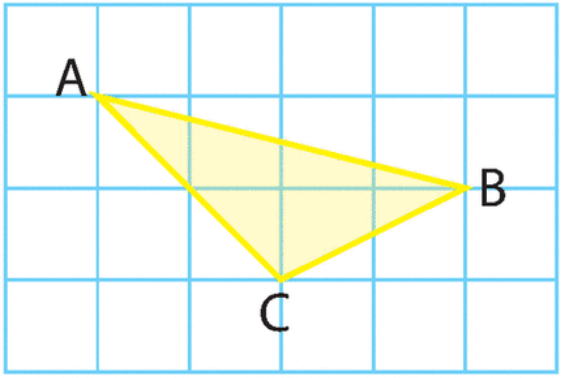
\includegraphics[scale=.35]{triangle-abc.png}
    \end{center}
  \end{minipage}
\end{exo}

\begin{exo}~\\
  \begin{minipage}[]{.6\textwidth}
    \begin{enumerate}
      \item À partir de la figure, citer un vecteur
      \begin{enumerate}
        \item opposé à $\vect{CD}$ ;
        \item de même direction et de même sens que $\vect{AC}$ ;
        \item de même direction que $\vect{BC}$ mais de sens contraire ;
        \item égal au vecteur $\vect{BA}$.
    \end{enumerate}
      \item Placer les points $E, F, G$ et $H$, images respectives du point $A$
        par les translations de vecteurs $\vect w$, $\vect v$, $\vect p$ et~$\vect m$.
      \item Placer les points $I, J, K$ et $L$, images respectives du point $B$
        par les translations de vecteurs $\vect r$, $\vect u$, $\vect w$ et~$\vect m$.
    \end{enumerate}
  \end{minipage}
  \begin{minipage}[]{.4\textwidth}
    \begin{center}
      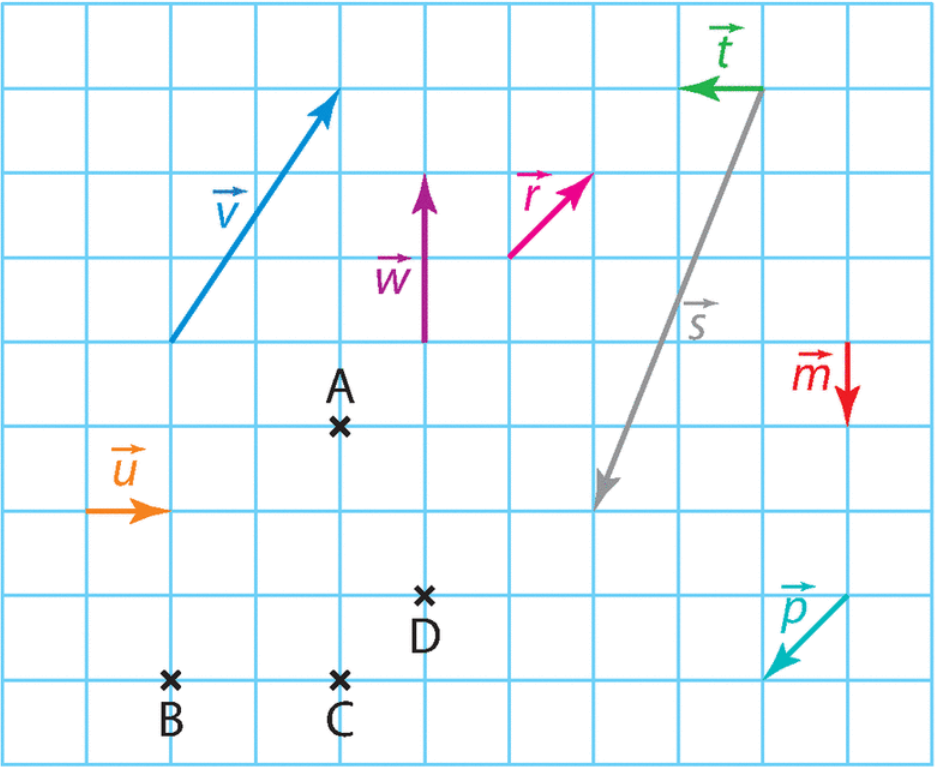
\includegraphics[scale=.2]{mucho-vectors.png}
    \end{center}
  \end{minipage}
\end{exo}

\begin{exo}~\\
  \begin{minipage}[]{.35\textwidth}
    On considère les vecteurs $\vect{AB}$ et $\vect{EF}$ et un point $C$.
    \begin{enumerate}
      \item Reproduire la figure sur papier quadrillé.
      \item Construire les points
        \begin{enumerate}
          \item $D$ tel que $\vect{CD}=\vect{AB}$ ;
          \item $G$ tel que $\vect{CG}=\vect{EF}$ ;
          \item $H$ tel que $\vect{HC}=\vect{AB}$ ;
          \item $I$ tel que $\vect{IC}=\vect{CG}$ ;
          \item $J$ tel que $\vect{BJ}=\vect{JC}$.
        \end{enumerate}
    \end{enumerate}
  \end{minipage}
  \begin{minipage}[]{.65\textwidth}
    \begin{center}
      \begin{tikzpicture}
        \foreach \x in {0, ..., 20}{
          \draw[opacity=.5] (.5*\x, -.1) -- (.5*\x, 5.1);
        }
        \foreach \y in {0, ..., 10}{
          \draw[opacity=.5] (-.1, .5*\y) -- (10.1, .5*\y);
        }

        \draw[very thick, -latex] (8, 4) -- (5,4);
        \draw[very thick, -latex] (6, 2.5) -- (5.5, 1);

        \point{6}{2.5}{black};
        \node at (6.25, 2.75) {$A$};

        \point{5.5}{1}{black};
        \node at (5.75, 1.25) {$B$};

        \point{3.5}{3}{black};
        \node at (3.75, 3.25) {$C$};

        \point{8}{4}{black};
        \node at (8.25, 4.25) {$E$};

        \point{5}{4}{black};
        \node at (5.25, 4.25) {$F$};
      \end{tikzpicture}
    \end{center}
  \end{minipage}
\end{exo}

\begin{exo}
  {\small On peut traduire de plusieurs façons une même situation. Recopier et compléter
  ce tableau.}
  \begin{center}
    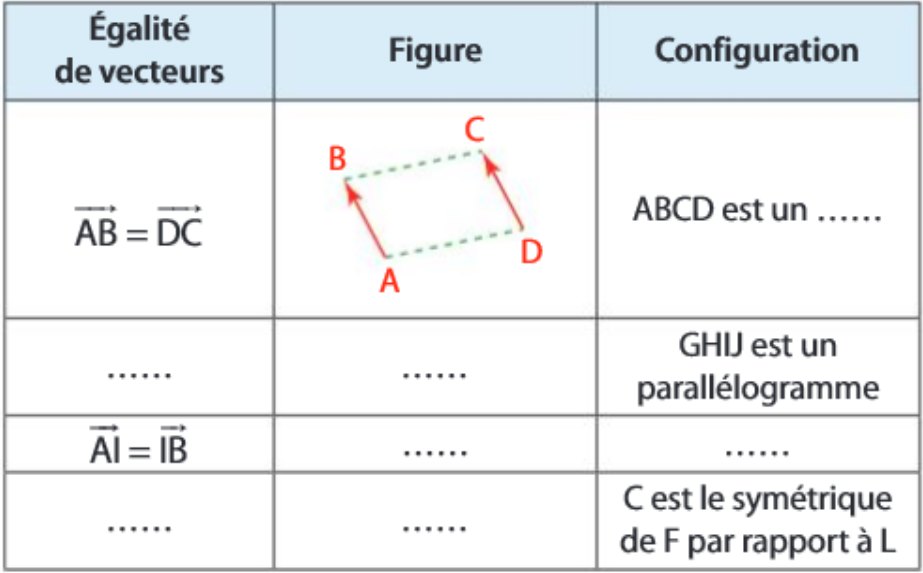
\includegraphics[scale=.5]{tableau.png}
  \end{center}
\end{exo}

\begin{exo}~\\
  \begin{minipage}[]{.35\textwidth}
    \begin{enumerate}
      \item Placer le point $M_1$ tel que
        \[
          \vect{AM_1} = \vect u+\vect v.
        \]
      \item Placer le point $M_2$ tel que 
        \[
          \vect{AM_2} = \vect v-\vect u.
        \]
    \end{enumerate}
  \end{minipage}
  \begin{minipage}[]{.65\textwidth}
    \begin{center}
      \begin{tikzpicture}
        \foreach \x in {0, ..., 10}{
          \draw[opacity=.5] (.5*\x, -.1) -- (.5*\x, 3.6);
        }
        \foreach \y in {0, ..., 7}{
          \draw[opacity=.5] (-.1, .5*\y) -- (5.1, .5*\y);
        }

        \draw[very thick, -latex] (.5, 3) -- node[above right] {$\vect{u}$}
        (2,2.5);
        \draw[very thick, -latex] (3.5, 1) -- node[left] {$\vect{v}$}
        (4.5,2.5);

        \point{.5}{1}{black};
        \node at (.75, 1.25) {$A$};
      \end{tikzpicture}
    \end{center}
  \end{minipage}
\end{exo}

\begin{exo}~\\[2mm]
  \begin{minipage}[]{.5\textwidth}
    \begin{enumerate}
      \item Tracer la somme $\vect a=\vect u+\vect v$.
      \item Tracer la somme $\vect b=\vect u+\vect w$.
      \item Tracer la somme $\vect c=\vect v+\vect w$.
      \item Tracer la différence $\vect d=\vect v-\vect v$.
      \item Tracer la différence $\vect e=\vect w-\vect v$.
      \item Tracer la différence $\vect f=\vect u-\vect w$.
    \end{enumerate}
  \end{minipage}
  \begin{minipage}[]{.5\textwidth}
    \begin{center}
      \begin{tikzpicture}
        \foreach \x in {0, ..., 6}{
          \draw[opacity=.5] (.5*\x, -.1) -- (.5*\x, 3.1);
        }
        \foreach \y in {0, ..., 6}{
          \draw[opacity=.5] (-.1, .5*\y) -- (3.1, .5*\y);
        }

        \draw[very thick, -latex] (0, .5) -- node[above left] {$\vect{u}$}
        (.5,1.5);
        \draw[very thick, -latex] (1, 2.5) -- node[above] {$\vect{v}$}
        (3,2.5);
        \draw[very thick, -latex] (2, 0) -- node[above] {$\vect{w}$}
        (1,.5);

      \end{tikzpicture}
    \end{center}
  \end{minipage}
\end{exo}

\begin{exo}~\\[-4mm]
  \begin{minipage}[]{.6\textwidth}
    \begin{enumerate}
      \item Reproduire la figure ci-contre.
      \item Construire un représentant de chacun des vecteurs suivants.
        \begin{align*}
          \textbf{a)}\;& -\vect r & 
          \textbf{b)}\;& \vect w+\vect r & 
          \textbf{c)}\;& \vect r+\vect v & 
          \textbf{d)}\;& \vect w-\vect r
        \end{align*}
    \end{enumerate}
  \end{minipage}
  \begin{minipage}[]{.4\textwidth}
    \begin{center}
      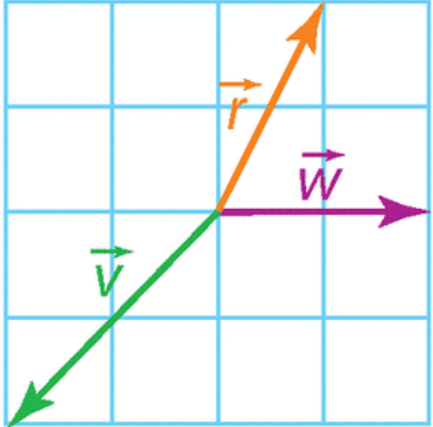
\includegraphics[scale=.25]{3d.png}
    \end{center}
  \end{minipage}
\end{exo}

\begin{exo}~\\[-4mm]
  \begin{minipage}[]{.4\textwidth}
    \begin{enumerate}
      \item Reproduire la figure ci-contre.
      \item Construire un représentant de chacun des vecteurs suivants.
        \begin{align*}
          \textbf{a)}\;& -\vect{BA} &
          \textbf{b)}\;& \vect{BC}+\vect{CD} \\
          \textbf{c)}\;& \vect{BA}+\vect{BC} &
          \textbf{d)}\;& \vect{CB}-\vect{BA} \\
          \textbf{e)}\;& \vect{DC}-\vect{DB} &
          &
        \end{align*}
    \end{enumerate}
  \end{minipage}
  \begin{minipage}[]{.6\textwidth}
    \begin{center}
      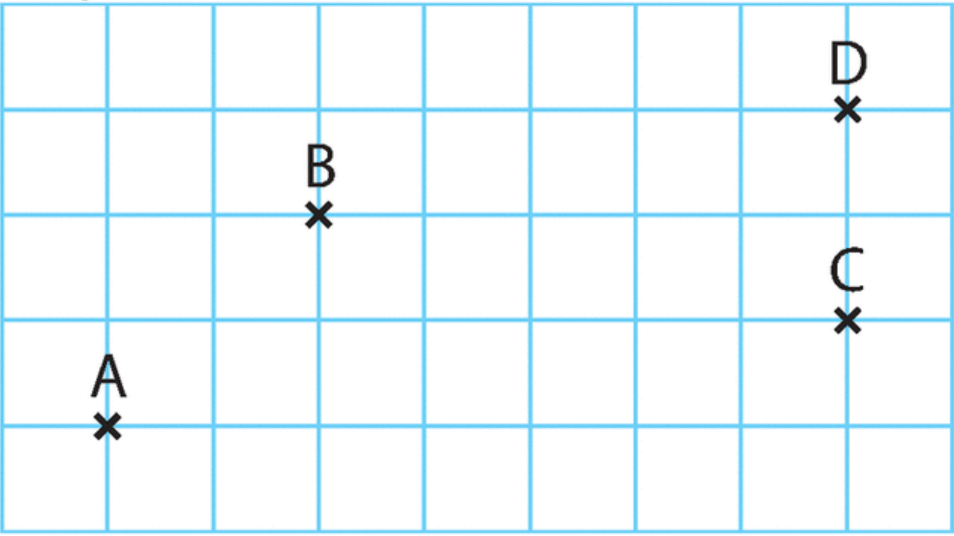
\includegraphics[scale=.25]{quad1.png}
    \end{center}
  \end{minipage}
\end{exo}

\begin{exo}~\\[-4mm]
  \begin{minipage}[]{.4\textwidth}
    \begin{enumerate}
      \item Reproduire la figure ci-contre.
      \item Construire un représentant de chacun des vecteurs suivants.
        \begin{align*}
          \textbf{a)}\;& \vect{AB}+\vect{CD} &
          \textbf{b)}\;& \vect{BA}+\vect{EF} \\
          \textbf{c)}\;& \vect{CD}+\vect{FE} &
          \textbf{d)}\;& \vect{EB}-\vect{AD}
        \end{align*}
    \end{enumerate}
  \end{minipage}
  \begin{minipage}[]{.6\textwidth}
    \begin{center}
      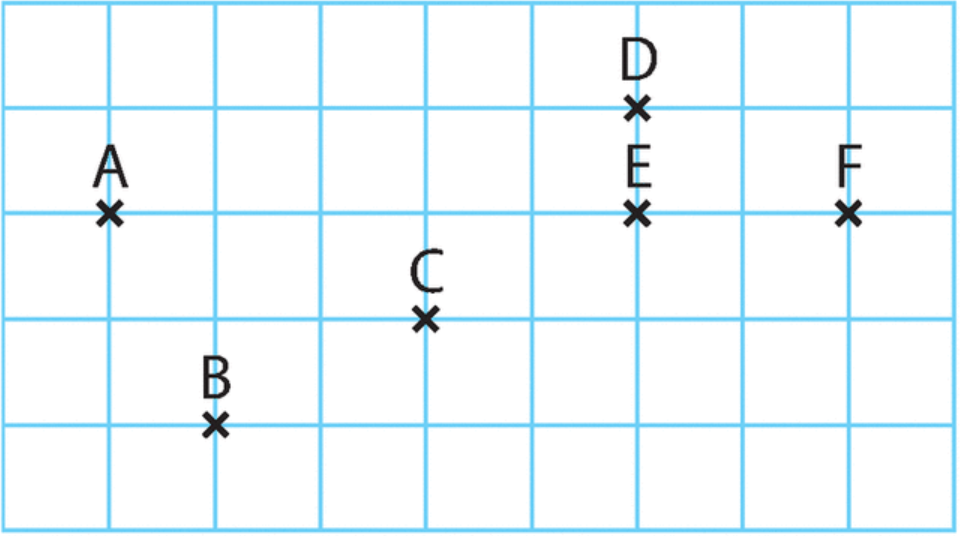
\includegraphics[scale=.25]{quad2.png}
    \end{center}
  \end{minipage}
\end{exo}

\begin{exo}~\\[-4mm]
  \begin{minipage}[]{.5\textwidth}
    En utilisant les points de la figure ci-contre, donner un vecteur égal à
    \begin{align*}
      \textbf{a)}\;& \vect{DE}+\vect{HI} &
      \textbf{b)}\;& \vect{GF}+\vect{CB} \\
      \textbf{c)}\;& \vect{AJ}-\vect{EI} &
      \textbf{d)}\;& \vect{BG}+\vect{GH} \\
      \textbf{e)}\;& \vect{BC}+\vect{CB}+\vect{BC} &
      \textbf{f)}\;& \vect{IJ}-\vect{CF}+\vect{JC}+\vect{FE} \\
      \textbf{g)}\;& \vect{AB}-\vect{CB} &
      \textbf{h)}\;& \vect{HF}-\vect{BC}+\vect{CD} %\\
%      \textbf{i)}\;& \vect{BD}+\vect{IH}-\vect{BH}-\vect{FD}
    \end{align*}
  \end{minipage}
  \begin{minipage}[]{.5\textwidth}
    \begin{center}
      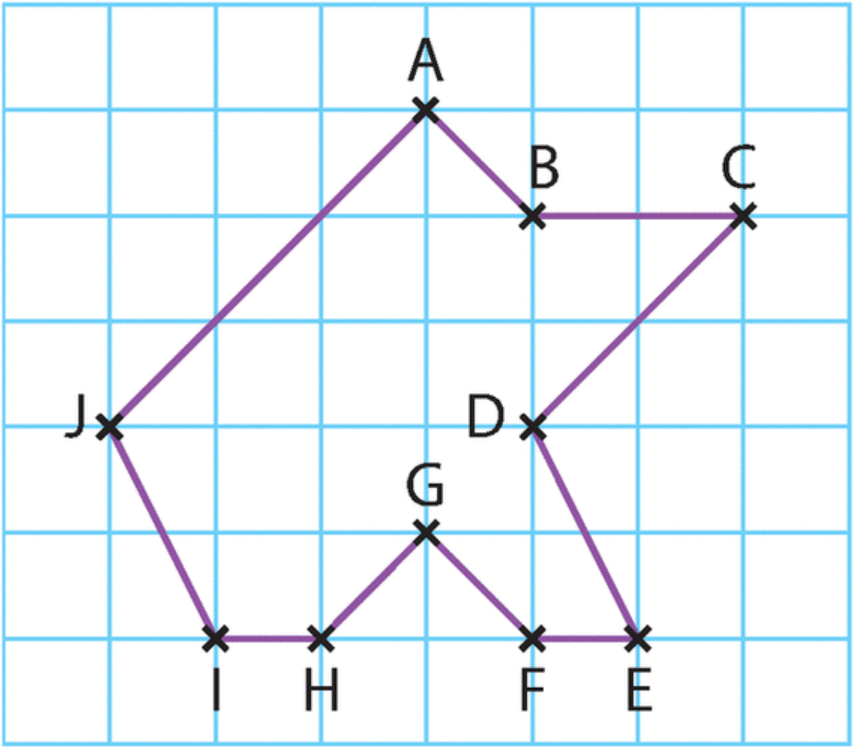
\includegraphics[scale=.2]{polygone.png}
    \end{center}
  \end{minipage}
\end{exo}

\begin{exo}~\\[-3mm]
  \begin{enumerate}
    \item Construire un carré $ABCD$ de centre $O$.
    \item Construire un représentant de chacun des vecteurs suivants.
      \begin{align*}
        \textbf{a)}\;& \vect u = \vect{AB}+\vect{OD} &
        \textbf{b)}\;& \vect w = \vect{AD}+\vect{OC} &
        \textbf{c)}\;& \vect z = \vect{AB}-\vect{AD}
      \end{align*}
  \end{enumerate}
\end{exo}

\begin{exo}
  Simplifier les expressions suivantes en utilisant la relation de Chasles.
  \begin{align*}
    \textbf{a)}\;& \vect{AC}+\vect{CB} &
    \textbf{c)}\;& \vect{AB}-\vect{CA}-\vect{CB} &
    \textbf{e)}\;& \vect{AC}-\vect{DC} \\
    \textbf{b)}\;& \vect{BC}+\vect{DB} &
    \textbf{d)}\;& \vect{AC}+\vect{CB}+\vect{BA} &
    \textbf{f)}\;& \vect{AB}-\vect{AC}+\vect{BC}-\vect{BA}
  \end{align*}
\end{exo}

\begin{exo}
  Recopier et compléter les égalités suivantes à l'aide de la relation de
  Chasles.
  \begin{align*}
    \textbf{a)}\;& \vect{IB} = \vect{\ldots A}+\vect{A\ldots} &
    \textbf{b)}\;& \vect{D\ldots} + \vect{C\ldots A}=\vect{\ldots B} &
    \textbf{c)}\;& \vect{HF} = \vect{HG} + \vect{\phantom{i}\!\ldots\!\phantom{i}} \\
    \textbf{d)}\;& \vect{E\ldots} + \vect{\ldots E} =
    \vect{\phantom i\!\ldots\!\phantom i} &
    \textbf{e)}\;& \vect{A\ldots} = \vect{A\ldots}+\vect{B \ldots} +
    \vect{CM} &
    \textbf{f)}\;& \vect{FE} + \vect{\phantom{i}\!\ldots\!\phantom{i}} = \vect0 \\
  \end{align*}
\end{exo}

\begin{exo}~\\[-5mm]
  \begin{minipage}[]{.65\textwidth}
  On donne la figure ci-dessous sur un quadrillage formé de carrés.
    \begin{enumerate}
      \item Citer un représentant du vecteur $\vect{AB}+\vect{BF}$.
      \item Citer deux représentants du vecteur $\vect{AC}+\vect{KE}$.
      \item Citer deux représentants du vecteur $\vect{AH}+\vect{IB}$.
      \item Citer un représentant du vecteur $\vect{IJ}+\vect{NC}$.
      \item Citer deux représentants du vecteur $\vect{LC}+\vect{DE}$.
    \end{enumerate}
  \end{minipage}
  \begin{minipage}[]{.35\textwidth}
    \begin{center}
      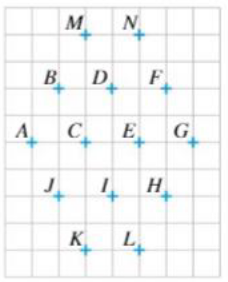
\includegraphics[scale=.5]{quad3.png}
    \end{center}
  \end{minipage}
\end{exo}

\begin{exo}~\\[-6mm]
  \begin{minipage}[]{.65\textwidth}
    Soient $ABCF$ et $FCDE$ deux parallélogrammes. Recopier et compléter les
    égalités suivantes à l'aide des points sur la figure.
    \begin{align*}
      \textbf{a)}\;& \vect{AB} - \vect{FD} = \vect{C\ldots} &
      \textbf{b)}\;& \vect{BF} + \vect{AC} = \vect{A\ldots} \\
      \textbf{c)}\;& \vect{DC} + \vect{JI} + \vect{CE} = \vect{\ldots A} &
      \textbf{d)}\;& \vect{IF} + \vect{JE} + \vect{IC} = \vect{\ldots J}
    \end{align*}
  \end{minipage}
  \begin{minipage}[]{.35\textwidth}
    \begin{center}
      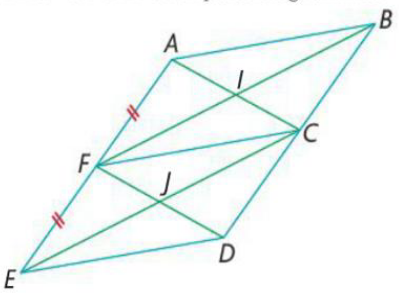
\includegraphics[scale=.4]{para.png}
    \end{center}
  \end{minipage}
\end{exo}

\begin{exo}~\\[-6mm]
  \begin{minipage}[]{.65\textwidth}
    Soient $BCDA$ et $BCFE$ deux parallélogrammes.
    \begin{enumerate}
      \item Démontrer que $ADFE$ est un parallélogramme.
      \item Soit $G$ le symétrique de $C$ par rapport à $B$.
        \begin{enumerate}
          \item Citer $3$ vecteurs égaux à $\vect{GB}$.
          \item Donner deux autres parallélogrammes à l'aide des points de la
            figure.
        \end{enumerate}
    \end{enumerate}
  \end{minipage}
  \begin{minipage}[]{.35\textwidth}
    \begin{center}
      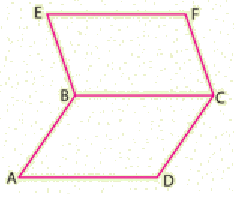
\includegraphics[scale=.7]{sym.png}
    \end{center}
  \end{minipage}
\end{exo}

\begin{exo}~\\[-5mm]
  \begin{enumerate}
    \item Représenter, sur une figure, un parallélogramme $ABCD$.
    \item Construire le point $N$ tel que $\vect{BN}=\vect{AC}$. Quelle est
      alors la nature du quadrilatère $CABN$ ?
    \item Construire le point $M$ tel que $M$ soit le symétrique de $B$ par
      rapport à $A$.
    \item \begin{enumerate}
        \item Donner $2$ vecteurs égaux au vecteur $\vect{AB}$. Que peut-on en
          déduire ?
        \item Quelle est alors la nature du quadrilatère $CMAN$ ? Justifier.
      \end{enumerate}
    \item Démontrer que $C$ est le milieu de $\left[ DN \right]$.
  \end{enumerate}
\end{exo}

\begin{exo}~\\[-8mm]
  \begin{minipage}[]{.6\textwidth}
    On considère les vecteurs suivants dans un repère orthonormé $(O; \vect i,
    \vect j)$.
    \begin{enumerate}
      \item Déterminer les coordonnées des vecteurs.
      \item Écrire les vecteurs en fonction de $\vect i$ et $\vect j$ comme
        l'exemple suivant :
        \[
          \vect{OB} = 3\vect i+2\vect j.
        \]
    \end{enumerate}
  \end{minipage}
  \begin{minipage}[]{.4\textwidth}
    \begin{center}
      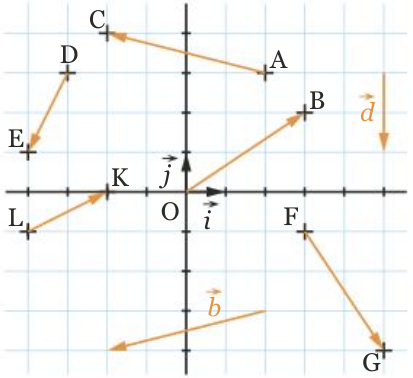
\includegraphics[scale=.4]{quad4.png}
    \end{center}
  \end{minipage}
\end{exo}

\begin{exo}
  On considère quatre points $E, F, G$ et $H$ dans un repère orthonormé $(O;
  \vect i, \vect j)$. Indiquer si $EFGH$ est un parallélogramme dans les
  différents cas.
  \begin{enumerate}
    \item $E(2; -1)$, $F(8; -1)$, $G(10; 3)$ et $H(4; 3)$
    \item $E(1; -1)$, $F(0; 2)$, $G(8; -3)$ et $H(7; 0)$
    \item $E(-2,06; -1,78)$, $F(0,92; -4,84)$, $G(9,22; -2,08)$ et $H(6,1; 1,3)$
    \item $E(3; -4)$, $F(14; -4)$, $G(10; 4)$ et $H(-1; 4)$
  \end{enumerate}
\end{exo}

\begin{exo}~\\%[-3mm]
  \begin{minipage}{.6\textwidth}
    Nami trouve la carte d'un trésor, accompagnée du parchemin
    suivant~:~«~Partant de A,
    \begin{itemize}
      \item $1$ à l'ouest, $1$ au sud ;
      \item $1$ à l'ouest, $2$ au sud ;
      \item $4$ à l'est, $1$ au nord ;
      \item $1$ à l'ouest, $3$ au sud ;
      \item $2$ à l'ouest. »
    \end{itemize}
    \begin{enumerate}
      \item Retrouver les différentes positions mentionnées dans le texte. On
        notera $A, B, C, D, E, F$ les points dans l'ordre de parcours.
    \end{enumerate}
  \end{minipage}
  \begin{minipage}{.4\textwidth}
    \begin{center}
      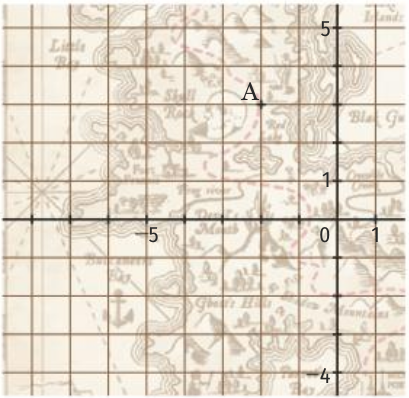
\includegraphics[scale=.4]{carte.png}
    \end{center}
  \end{minipage}
  \begin{enumerate}
      \setcounter{enumi}{1}
    \item Donner les coordonnées des vecteurs $\vect{AB}, \vect{BC},
      \vect{CD}, \vect{DE}$ et $\vect{EF}$.
    \item En utilisant la même notation que celle du parchemin, quel déplacement
      Nami doit-elle effectuer afin de passer de $A$ à $F$ directement ?
  \end{enumerate}
\end{exo}

\begin{exo}
  On considère les points suivants dans un repère orthonormé $(O; \vect i, \vect
  j)$ : $A(-4; -3)$, $B(4; -2)$, $C(3; 2)$, $D(-5; 1)$ et $E(2; 6)$. Répondre
  aux questions à l'aide des vecteurs, en expliquant la démarche.
  \emph{Vous pouvez faire une figure pour avoir un idée de la réponse.}
  \begin{enumerate}
    \item Quelle est la nature du quadrilatère $ABCD$ ?
    \item Que représente le point $C$ pour le segment $\left[ BE \right]$ ?
    \item Le point $C$ est-il l'image du point $E$ par la translation de vecteur
      $\vect{DA}$ ?
  \end{enumerate}
\end{exo}

\begin{exo}~\\[-3mm]
  \begin{minipage}[]{.6\textwidth}
    On considère les points et les vecteurs suivants dans un repère $(O; \vect
    i, \vect j)$.
    \begin{enumerate}
      \item Calculer les coordonnées de $\vect u$ telles que $\vect
        u=\vect{AB}+\vect{CD}$. Construire le point $I$ tel que
        $\vect{OI}=\vect u$.
      \item Calculer les coordonnées de $\vect w$ telles que $\vect
        w=\vect{AB}+\vect{EF}$. Construire le point $J$ tel que
        $\vect{OJ}=\vect w$.
      \item Calculer les coordonnées de $\vect t$ telles que $\vect
        t=\vect{CD}+\vect{EF}$. Construire le point $H$ tel que
        $\vect{OH}=\vect t$.
    \end{enumerate}
  \end{minipage}
  \begin{minipage}[]{.4\textwidth}
    \begin{center}
      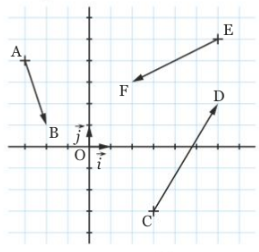
\includegraphics[scale=.6]{quad5.png}
    \end{center}
  \end{minipage}
\end{exo}

\end{document}
